\chapter{映射}

\section{连续映射}

\begin{definition}{连续映射}
    设$X,Y$是拓扑空间，$f:X\to Y$是一个映射. 如果对$Y$中任意开集$V$，其原像$f^{-1}(V)$在$X$中是开集，则称$f$是\textbf{连续的}.
\end{definition}

\begin{instance}
    \begin{enumerate}
        \item 恒等映射 $\setjot[-10]\begin{aligned}[t]
            \mathrm{id}:X &\to X \\ 
            x &\mapsto x
        \end{aligned}$ 是连续的.
        \item 常值映射 $\setjot[-10]\begin{aligned}[t]
            c:X&\to Y \\ 
            x&\mapsto y_0
        \end{aligned}$ 是连续的.
        \item $X$是拓扑空间，$A\subset X$，则包含映射 $\setjot[-10]\begin{aligned}[t]
            i:A &\to X \\ 
            x&\mapsto x
        \end{aligned}$ (其中$A$是$X$的子空间) 是连续的.
        \item $X,Y$是拓扑空间，在乘积空间$X\times Y$上投射 $\setjot[-10]\begin{aligned}[t]
            \pi_1:X\times Y &\to X \\ 
            (x,y)&\mapsto x
        \end{aligned}$ 和 $\setjot[-10]\begin{aligned}[t]
            \pi_2:X\times Y &\to Y \\ 
            (x,y)&\mapsto y
        \end{aligned}$ 是连续的.
    \end{enumerate}
\end{instance}

\begin{lemma}
    若$f:X\to Y$和$g:Y\to Z$是连续映射，则复合映射$g\circ f:X\to Z$也是连续的.
\end{lemma}
\begin{proof}
    $\forall\,\open V\in Z$，$(g\circ f)^{-1}(V)=f^{-1}(g^{-1}(V))$.\par 
    因为$g$连续，$g^{-1}(V)$是$Y$中的开集.又因为$f$连续，$f^{-1}(g^{-1}(V))$是$X$中的开集.
\end{proof}

\begin{instance}
    $f:X\to Y$是连续映射，$A\subset X$，则$f|_A：A\to Y$是连续的.\par
        \begin{wrapfigure}{r}{0.25\textwidth}
        \vspace{-2.8 em}
        \begin{tikzcd}[column sep=2.4em, row sep=1.8em,every label/.append style={font=\normalsize},font=\normalsize]
            A \arrow[rr, "f|_A"] \arrow[rd, "i"'] &                    & Y \\
                                      & X \arrow[ru, "f"'] &  
        \end{tikzcd}
        \vspace{-2 em}
    \end{wrapfigure}
    回顾之前的内容，限制映射有如右图所示的交换图，即$f|_A=f\circ i$.\par
    又$f$和$i$都是连续的，因此$f|_A$也是连续的.
\end{instance}

\begin{lemma}
    设$f:X\to Y$是一个映射，$\mcal{B}$是$Y$的一个拓扑基，则$f$是连续的$\Leftrightarrow \forall\, B\in\mcal{B},f^{-1}(B)$是$X$中的开集.
\end{lemma}
这个定理的证明只需要利用连续映射的定义和拓扑基生成拓扑的方式即可完成.\par
这一引理让我们不必讨论$Y$中所有开集的原像，只需讨论基元素的原像.\par

\begin{instance}
    (1)\; $\setjot[-10]\begin{aligned}[t]
        f: \mb{E}^1 &\to \mb{E}^1 \\
        x &\mapsto f(x)=x^n,e^x,\ln{x},\sin{x},\cos{x}
    \end{aligned}$都是连续函数.\par
    (2)\; $\setjot[-10]\begin{aligned}[t]
        f:\mb{E}^2 &\to \mb{E}^1 \\
        (x,y) &\mapsto f(x,y)=x+y,x-y,xy,\frac{x}{y}(y\neq 0)
    \end{aligned}$都是连续函数.
\end{instance}

\begin{lemma}
    $f:X\to Y$是一个映射，则$f$是连续的$\Leftrightarrow \forall\,\close C\in Y,f^{-1}(C)$是$X$中的闭集.
\end{lemma}
这个引理相较于连续映射最初始的定义，只是将其中的开集改为闭集.成立的原因是开集取补就是闭集.\par

\begin{proposition}
    设$f:X\to Y_1\times Y_2$是一个映射，定义为$f(x)=(f_1(x),f_2(x))$，其中$f_1:X\to Y_1, f_2:X\to Y_2$. 则$f$连续$\Leftrightarrow f_1$和$f_2$都连续.
\end{proposition}
\begin{proof}
    “$\Rightarrow$” 投射$\setjot[-10]\begin{aligned}[t]
            \pi_1:X\times Y &\to X \\ 
            (x,y)&\mapsto x
        \end{aligned}$ 和 $\setjot[-10]\begin{aligned}[t]
            \pi_2:X\times Y &\to Y \\ 
            (x,y)&\mapsto y
        \end{aligned}$都是连续的.\par
    $f_1=\pi_1\circ f, f_2=\pi_2\circ f$. 由于投射和$f$是连续的，所以$f_1,f_2$都连续.\par
    “$\Leftarrow$” $\mcal{B}=\{U_1\times U_2|U_i\text{是}Y_i\text{中的开集}\}$是$Y_1\times Y_2$的一个拓扑基.\par
    $f^{-1}(U_1\times U_2)= f_1^{-1}(U_1)\cap f_2^{-1}(U_2)$. 由于$f_1,f_2$连续，$f_1^{-1}(U_1)$和$f_2^{-1}(U_2)$都是$X$中的开集.\par
    因此$f^{-1}(U_1\times U_2)$是$X$中的开集.
\end{proof}

\begin{lemma}{粘贴引理 (Pasting Lemma)}
    $X$是一个拓扑空间，$A,B$是$X$中的闭集且$X=A\cup B$.设$f:A\to Y$和$g:B\to Y$是两个连续映射，且对任意$x\in A\cap B$都有$f(x)=g(x)$. 则由它们定义的映射
    \[h:X\to Y, x\mapsto\begin{cases} f(x) & x\in A \\ g(x) & x\in B \end{cases}\]
    是连续的.
\end{lemma}
\begin{figure}[h]
    \centering
    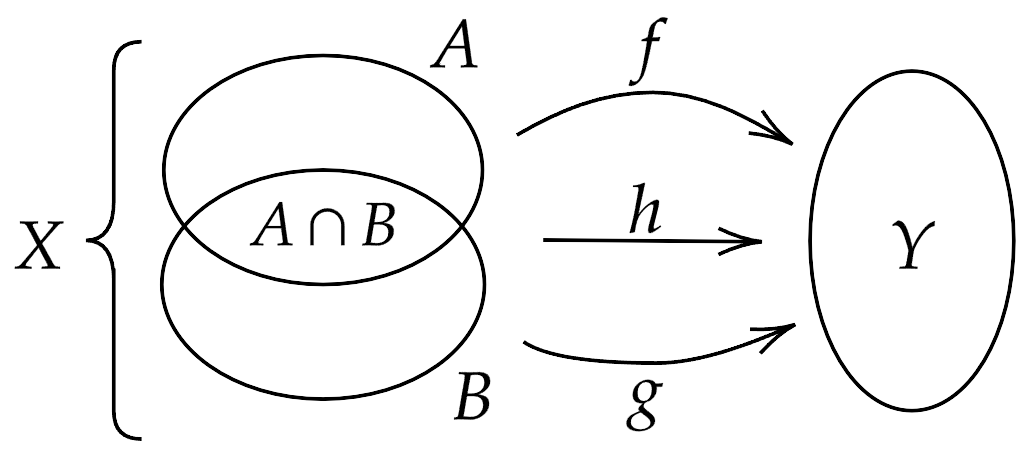
\includegraphics[width=0.4\textwidth]{fig/2.12.png}
    \captionof{figure}{粘贴引理示意图}
\end{figure}
\begin{proof}
    $\forall\,\close C\in Y$，则$f^{-1}(C)$是$A$中的闭集，$g^{-1}(C)$是$B$中的闭集，且$h^{-1}(C)=f^{-1}(C)\cup g^{-1}(C)$.\par
    根据定义，$\exists\,\close D_1\in X,\st f^{-1}(C)=D_1\cap A$.\par
    同理，$\exists\,\close D_2\in X,\st g^{-1}(C)=D_2\cap B$.\par
    因为$A,B$都是$X$中的闭集，$f^{-1}(C)$和$g^{-1}(C)$都是$X$中的闭集，因此$h^{-1}(C)=f^{-1}(C)\cup g^{-1}(C)$也是$X$中的闭集.
\end{proof}

\section{同胚}

\begin{definition}{同胚}
    设 $X,Y$ 是拓扑空间，$f:X\to Y$ 是一个具有逆映射 $f^{-1}:Y\to X$ 的双射.
    如果 $f$ 和 $f^{-1}$ 都是连续的, 则称 $f$ 是一个\textbf{同胚}.
    如果存在一个在 $X$ 和 $Y$ 之间的同胚, 则称 $X$ 和 $Y$ 是\textbf{同胚的}, 记作 $X\cong Y$.
\end{definition}

\begin{remark}
    设 $f:X\cong Y$. 那么 $f$ 是 $X$ 中的点与 $Y$ 中的点之间的一个双射. $f$ 导出 $X$ 中的开集与 $Y$ 中的开集之间的一个双射.
    \begin{enumerate}[(i)]
        \item $\forall\, U$ 是 $X$ 中的开集, 则 $f(U)$ 是 $Y$ 中的开集.
        ($f^{-1}:Y\to X$ 是连续的 $\Rightarrow (f^{-1})^{-1}(U)$ 在 $Y$ 中是开集, 即 $f(U)$ 在 $Y$ 中是开集)
        \item $\forall\, V$ 是 $Y$ 中的开集, 则 $f^{-1}(V)$ 是 $X$ 中的开集.
        ($f:X\to Y$ 是连续的 $\Rightarrow f^{-1}(V)$ 在 $X$ 中是开集)
    \end{enumerate}
\end{remark}

\begin{proposition}
    关系“$\cong$”是拓扑空间之间的一个等价关系.
    \begin{enumerate}[(i)]
        \item $X\cong X$
        \item $X\cong Y \Rightarrow Y\cong X$
        \item $X\cong Y, Y\cong Z \Rightarrow X\cong Z$
    \end{enumerate}
\end{proposition}

\begin{instance}
    \begin{enumerate}
        \item $(-1,1)\subset \mb{E}^1, (-1,1)\cong \mb{E}^1$.
        $f:(-1,1)\to\mb{E}^1, x\mapsto \frac{x}{1-|x|}$.
        $f^{-1}:\mb{E}^1\to(-1,1), y\mapsto \frac{y}{1+|y|}$.

        \item $\mathring{D}^n = \{(x_1,\dots,x_n)\in\mb{E}^n | x_1^2+\dots+x_n^2 < 1\}$. 则 $\mathring{D}^n \cong \mb{E}^n$.
        $f:\mathring{D}^n\to\mb{E}^n, x\mapsto \frac{x}{1-\|x\|}$.
        $f^{-1}:\mb{E}^n\to\mathring{D}^n, y\mapsto \frac{y}{1+\|y\|}$.
        其中 $\|x\|=\sqrt{x_1^2+\dots+x_n^2}$.

        \item $\mathring{C}^n = \{(x_1,\dots,x_n)\in\mb{E}^n | |x_i|<1, i=1,\dots,n\}$. 则 $\mathring{C}^n \cong \mb{E}^n$.
        $f:\mathring{C}^n\to\mb{E}^n, (x_1,\dots,x_n)\mapsto (\frac{x_1}{1-|x_1|},\dots,\frac{x_n}{1-|x_n|})$.
        $f^{-1}:\mb{E}^n\to\mathring{C}^n, (y_1,\dots,y_n)\mapsto (\frac{y_1}{1+|y_1|},\dots,\frac{y_n}{1+|y_n|})$.

        \item $\mathring{D}^n \cong \mathring{C}^n$.

        \item (i) $(a,b)\cong(-\infty,c)\cong(d,+\infty)\cong\mb{E}^1$.
        (ii) $[a,b)\cong[c,d)\cong(-\infty,e]\cong[f,+\infty)$.
        (iii) $[a,b]\cong[c,d]$.

        \item $\mb{E}^n-\{0\} \cong \mb{E}^n-D^n$.
        $f:\mb{E}^n-\{0\}\to\mb{E}^n-D^n, x\mapsto x+\frac{x}{\|x\|}$.
        $f^{-1}:\mb{E}^n-D^n\to\mb{E}^n-\{0\}, y\mapsto y-\frac{y}{\|y\|}$.

        \item $S^2=\{(x_1,x_2,x_3)\in\mb{E}^3 | x_1^2+x_2^2+x_3^2=1\}$.
        令 $N=(0,0,1)\in S^2$. 则 $S^2-\{N\}\cong\mb{E}^2$. 这被称为\textbf{球极投影}.
        $f:S^2-\{N\}\to\mb{E}^2, (x_1,x_2,x_3)\mapsto(\frac{2x_1}{1-x_3},\frac{2x_2}{1-x_3},-1)$.
        $f^{-1}:\mb{E}^2\to S^2-\{N\}, (y_1,y_2)\mapsto(\frac{2y_1}{y_1^2+y_2^2+1},\frac{2y_2}{y_1^2+y_2^2+1},\frac{y_1^2+y_2^2-1}{y_1^2+y_2^2+1})$.

        \item $S^n\subset\mb{E}^{n+1}$. $S^n-\{\text{pt}\}\cong\mb{E}^n, n\ge 1$.
    \end{enumerate}
\end{instance}

\begin{definition}{开映射和闭映射}
    映射 $f:X\to Y$ 称为\textbf{开映射} (相应地, \textbf{闭映射})，如果 $f$ 将 $X$ 中的每个开集 (相应地, 闭集) 映射到 $Y$ 中的一个开集 (相应地, 闭集).
\end{definition}

\begin{remark}
    同胚 $f:X\cong Y$ 既是开映射也是闭映射.
\end{remark}

\begin{instance}
    投射 $\pi_1:X\times Y\to X, (x,y)\mapsto x$ 是开映射.
\end{instance}

\begin{proposition}
    设 $X,Y$ 是拓扑空间. $f:X\to Y$ 是一个同胚 $\Leftrightarrow$ $f$ 是双射、连续且开 $\Leftrightarrow$ $f$ 是双射、连续且闭.
\end{proposition}
\begin{proof}
    “$\Rightarrow$” $\forall$ 开集 $U\subset X$, 因为 $f^{-1}:Y\to X$ 是连续的, $(f^{-1})^{-1}(U)$ 在 $Y$ 中是开集, 即 $f(U)$ 在 $Y$ 中是开集. 所以 $f$ 是一个开映射.
    “$\Leftarrow$” $\forall$ 开集 $U\subset X$, 因为 $f:X\to Y$ 是开映射, $f(U)$ 在 $Y$ 中是开集. $f(U)=(f^{-1})^{-1}(U)$. 所以 $f^{-1}:Y\to X$ 是连续的.
\end{proof}

\begin{theorem}
    如果 $f:X\to Y$ 是一个同胚且 $X$ 是Hausdorff空间, 那么 $Y$ 也是Hausdorff空间.
\end{theorem}
\begin{proof}
    $\forall\, y_1,y_2\in Y, y_1\neq y_2$. 则 $f^{-1}(y_1)\neq f^{-1}(y_2)$.
    因为 $X$ 是Hausdorff空间, 存在不相交的开集 $U_1, U_2$ 使得 $f^{-1}(y_1)\in U_1, f^{-1}(y_2)\in U_2$.
    由于 $f$ 是同胚, $f(U_1)$ 和 $f(U_2)$ 是 $Y$ 中的开集, 且 $y_1\in f(U_1), y_2\in f(U_2)$.
    $f(U_1)\cap f(U_2) = f(U_1\cap U_2) = f(\emptyset) = \emptyset$.
    因此 $Y$ 是Hausdorff空间.
\end{proof}

\begin{instance}
    $\mb{E}^1\not\cong \mb{R}_{fc}$ (有限补拓扑). 因为 $\mb{E}^1$ 是Hausdorff空间, 而 $\mb{R}_{fc}$ 不是.
\end{instance}

\begin{definition}{拓扑性质}
    一个拓扑空间的性质, 如果在同胚下保持不变, 则称之为一个\textbf{拓扑性质}.
\end{definition}

\subsection{嵌入}

\begin{definition}{嵌入}
    $X$ 在 $Y$ 中的一个\textbf{嵌入}是一个连续映射 $f:X\to Y$, 它将 $X$ 同胚地映射到子空间 $f(X)\subset Y$ 上.
\end{definition}

\begin{remark}
    嵌入是单射.
\end{remark}

\begin{instance}
    $f:S^1\to\mb{E}^2$ 是一个嵌入.
\end{instance}

\begin{proposition}
    设 $X,Y$ 是拓扑空间. $f:X\to Y$ 是一个嵌入
    $\Leftrightarrow$ $f$ 是单射、连续的, 并且 $f:X\to f(X)$ 是开映射.
    $\Leftrightarrow$ $f$ 是单射、连续的, 并且 $f:X\to f(X)$ 是闭映射.
\end{proposition}

\begin{instance}
    $f:S^1\to\mb{E}^3$ 是一个嵌入, 称为一个\textbf{纽结 (Knot)}.
\end{instance}

\begin{definition}{同痕}
    设 $f_0, f_1: S^1 \to \mb{E}^3$ 是两个嵌入. 如果存在一个连续映射 $F:S^1\times[0,1]\to\mb{E}^3$, 使得
    $F(x,0)=f_0(x)$, $F(x,1)=f_1(x)$, 并且对于任意 $t\in[0,1]$, 映射 $f_t=F(\cdot,t):S^1\to\mb{E}^3$ 都是一个嵌入,
    那么称 $f_0$ 和 $f_1$ 是\textbf{同痕的 (isotopic)}.
\end{definition}

\begin{instance}
    下图中的两个纽结是同痕的.
\end{instance}

\begin{instance}
    $f:S^1\to T^2$ 的嵌入.
\end{instance}

\begin{instance}
    $S^1\times[0,1]\subset \mb{E}^2$ 是一个圆环.
    $f:S^1\times[0,1]\to\mb{E}^3$ 是一个嵌入.
\end{instance}

\chapter{度量空间}

\section{度量和度量拓扑}

\begin{definition}{度量}
    设 $X$ 是一个集合. $X$ 上的一个\textbf{度量}是一个函数 $d:X\times X\to \mb{R}$ 满足:
    \begin{enumerate}[(i)]
        \item $d(x,y)\ge 0$, “=”成立 $\Leftrightarrow x=y$.
        \item $d(x,y)=d(y,x)$. (对称性)
        \item $d(x,y)+d(y,z)\ge d(x,z)$. (三角不等式)
    \end{enumerate}
    偶对 $(X,d)$ 称为一个\textbf{度量空间}.
\end{definition}

\begin{instance}
    \begin{enumerate}
        \item $\mb{R}^n$, $x=(x_1,\dots,x_n), y=(y_1,\dots,y_n)$.
        $d(x,y)=\sqrt{(x_1-y_1)^2+\dots+(x_n-y_n)^2}$. (欧几里得度量)
        \item $\mb{R}^n$, $d_1(x,y)=|x_1-y_1|+\dots+|x_n-y_n|$. (出租车度量)
        \item 设 $X\neq\emptyset$ 是一个集合.
        $d(x,y)=\begin{cases} 0, & \text{if } x=y \\ 1, & \text{if } x\neq y \end{cases}$. 这称为\textbf{离散度量}.
    \end{enumerate}
\end{instance}

\begin{definition}{度量拓扑}
    $\forall x\in (X,d)$, 开球 $B(x,\varepsilon)=\{y\in X | d(x,y)<\varepsilon\}$.
    集合 $\mcal{B}=\{B(x,\varepsilon)|x\in X, \varepsilon>0\}$ 是 $X$ 上的一个拓扑的基.
    这个拓扑称为由度量 $d$ \textbf{诱导的度量拓扑}.
\end{definition}

\begin{proof}[$\mcal{B}$ 是一个基的证明]
    (a) $\forall x\in X$, $x\in B(x,\varepsilon)$, 所以 $X=\bigcup_{x\in X}B(x,\varepsilon)$.
    (b) 设 $x\in B(x_1,\varepsilon_1)\cap B(x_2,\varepsilon_2)$.
    则 $d(x,x_1)<\varepsilon_1$ 且 $d(x,x_2)<\varepsilon_2$.
    取 $0<\varepsilon < \min\{\varepsilon_1-d(x,x_1), \varepsilon_2-d(x,x_2)\}$.
    则 $B(x,\varepsilon)\subset B(x_1,\varepsilon_1)\cap B(x_2,\varepsilon_2)$.
    因为 $\forall y\in B(x,\varepsilon)$, $d(y,x_1)\le d(y,x)+d(x,x_1) < \varepsilon+d(x,x_1) < \varepsilon_1-d(x,x_1)+d(x,x_1)=\varepsilon_1$.
    所以 $y\in B(x_1,\varepsilon_1)$.
    同理 $y\in B(x_2,\varepsilon_2)$.
\end{proof}

\begin{example}
    离散度量诱导了 $X$ 上的离散拓扑.
    $B(x,\varepsilon) = \begin{cases} \{x\}, & \text{if } \varepsilon\le 1 \\ X, & \text{if } \varepsilon > 1 \end{cases}$.
    基 $\mcal{B}=\{B(x,\varepsilon)|x\in X, \varepsilon>0\}$ 生成了 $X$ 上的离散拓扑.
\end{example}

\begin{proposition}
    每个度量空间都是Hausdorff空间.
\end{proposition}
\begin{proof}
    假设 $(X,d)$ 是一个度量空间, $x_1,x_2$ 是 $X$ 中两个不同的点.
    那么 $d(x_1,x_2)>0$. 令 $\varepsilon = \frac{1}{3}d(x_1,x_2)$.
    那么 $B(x_1,\varepsilon)$ 和 $B(x_2,\varepsilon)$ 分别是 $x_1,x_2$ 的邻域.
    并且 $B(x_1,\varepsilon)\cap B(x_2,\varepsilon)=\emptyset$.
    (反证) 假设 $y\in B(x_1,\varepsilon)\cap B(x_2,\varepsilon)$.
    那么 $d(x_1,x_2)\le d(x_1,y)+d(y,x_2) < 2\varepsilon = \frac{2}{3}d(x_1,x_2)$. 矛盾!
\end{proof}

\begin{corollary}
    度量空间中的每个单点集都是闭集.
\end{corollary}

\begin{definition}{可度量化}
    $X$ 是一个拓扑空间. 我们说 $X$ 是\textbf{可度量化的}, 如果在 $X$ 上存在一个度量 $d$ 诱导了 $X$ 上的拓扑.
\end{definition}

\begin{instance}
    \begin{enumerate}
        \item 离散拓扑是可度量化的.
        \item 如果 $X$ 不是Hausdorff空间, 那么 $X$ 是不可度量化的. 例如, $\mb{R}_{fc}$ (有限补拓扑)是不可度量化的.
    \end{enumerate}
\end{instance}

\begin{question}
    设 $d$ 和 $d'$ 是 $X$ 上的两个度量. 它们诱导的度量拓扑为 $\mcal{T}_d$ 和 $\mcal{T}_{d'}$.
    $\mcal{T}_d = \mcal{T}_{d'}$? (参考 Munkres 引理 20.2)
\end{question}